\documentclass{article}

\usepackage{geometry}
\usepackage{makecell}
\usepackage{array}
\usepackage{multicol}
\usepackage{setspace}
\usepackage{changepage}
\usepackage{booktabs}
\usepackage[explicit]{titlesec}
\usepackage{hyperref}
\usepackage{graphicx}
\usepackage{cprotect}
\usepackage{float}
\newcolumntype{?}{!{\vrule width 1pt}}
\newcommand{\paragraphlb}[1]{\paragraph{#1}\mbox{}\\}
\newcommand{\subparagraphlb}[1]{\subparagraph{#1}\mbox{}\\}
\renewcommand{\contentsname}{Inhaltsverzeichnis:}
\renewcommand\theadalign{tl}
\makeatletter
\newcommand{\Spvek}[2][r]{%
  \gdef\@VORNE{1}
  \left(\hskip-\arraycolsep%
    \begin{array}{#1}\vekSp@lten{#2}\end{array}%
  \hskip-\arraycolsep\right)}

\def\vekSp@lten#1{\xvekSp@lten#1;vekL@stLine;}
\def\vekL@stLine{vekL@stLine}
\def\xvekSp@lten#1;{\def\temp{#1}%
  \ifx\temp\vekL@stLine
  \else
    \ifnum\@VORNE=1\gdef\@VORNE{0}
    \else\@arraycr\fi%
    #1%
    \expandafter\xvekSp@lten
  \fi}
\makeatother
\setstretch{1.10}
\setlength{\parindent}{0pt}
\setcounter{tocdepth}{5}

\titleformat{\section}
  {\normalfont\Large\bfseries}{\thesection}{1em}{\hyperlink{sec-\thesection}{#1}
\addtocontents{toc}{\protect\hypertarget{sec-\thesection}{}}}
\titleformat{name=\section,numberless}
  {\normalfont\Large\bfseries}{}{0pt}{#1}

\titleformat{\subsection}
  {\normalfont\large\bfseries}{\thesubsection}{1em}{\hyperlink{subsec-\thesubsection}{#1}
\addtocontents{toc}{\protect\hypertarget{subsec-\thesubsection}{}}}
\titleformat{name=\subsection,numberless}
  {\normalfont\large\bfseries}{\thesubsection}{0pt}{#1}

\hypersetup{
    colorlinks,
    citecolor=black,
    filecolor=black,
    linkcolor=black,
    urlcolor=black
}

\geometry{top=12mm, left=1cm, right=2cm}
\title{\vspace{-1cm}Mathematik für Informatik 2}
\author{Andreas Hofer}

\begin{document}
	\maketitle
	\tableofcontents
	\section{Kombinatorik}
	Die Kombinatorik ist die Vorstufe der Wahrscheinlichkeitstheorie und beantwortet allgemeine Fragen des Abzählens. Zum Beispiel, wenn man wissen will wie viele Möglichkeiten es gibt Objekte anzuordnen und auszuwählen. Zum Beispiel wenn man eine bestimmte Menge an möglichen Ausgängen ermitteln will (Die Menge an verschiedenen Würfelpositionen). Dabei unterscheidet man zwischen den günstigen und den möglichen Fällen. Günstige Fälle sind jene die man erhalten will, während die möglichen Fälle die Summe aller Fälle ist. Ein spezieller Fall der Wahrscheinlichkeit ist das Laplace-Experiment, in welchem jeder Ausgang die gleiche Wahrscheinlichkeit hat. (Zum Beispiel ein Würfel, welcher stets eine Chance von 1/6 hat).
	\subsection{Abzählverfahren}
	Bei den Abzählverfahren der Kombinatorik existieren drei fundamentale Regeln:
	\subsubsection{Summenregel}
	Bei zwei endlichen disjunkten (Mengen ohne gemeinsame Elemente) Mengen gilt, dass die Vereinigung der Mengen die selbe Mächtigkeit hat als die Summe dieser zwei Mengen: $|A \cup B|=|A|+|B|$. Die Union der Mengen hat somit die gleiche Menge an Elementen, als die Summe der beiden Mengen. Das ist relevant in Fällen, in denen Eigenschaften eines Objektes sich einander ausschließen. Zum Beispiel kann man ein Auto nur entweder als Kleinwagen oder als Mittelklassewagen klassifizieren, jedoch nie beides.
	\paragraphlb{Verallgemeinerung}
	Für diese Regel existiert auch einen Verallgemeinerung, bei der mehr als zwei Mengen verwendet werden kann. Eine Regel dabei ist, dass der Schnitt jeder Menge die leere Menge ergibt.
	\subsubsection{Produktregel}
	Anders als bei der Summenregel müssen bei der Produktregel die Mengen nicht disjunkt sein. Hierbei wird das kartesische Produkt der Mengen gebildet: $|AxB|=|A|\point|B|$. Ein Beispiel zur Anwendung ist die Routenplanung. Angenommen es gibt drei Routen von Wien nach Graz und 4 Routen von Wien nahc Marburg, kann man diese kombinieren, da man eine beliebige Route von Wien nach Graz und eine beliebige Route von Graz nach Marburg verwenden kann. So gibt es ingsesamt 12 verschiedene Möglichkeiten von Wien nach Marburg zu kommen, da man jede der ersten Route mit jeder der zweiten Route kombinieren kann.
	\paragraphlb{Verallgemeinerung}
	Auch bei der Produktregel existiert eine Verallgemeinerung mit beliebig vielen Schritten. Dabei wird wieder die Mächtigkeit jeder Teilmenge mit jeder anderen Teilmenge multipliziert. Ein Beispiel dafür ist die Menge der Möglichkeiten bei einer Binärzahl. So hat man 8 Bits zur Verfügung und jedes Bit kann zwei Mögliche Zustände (1 und 0) besitzen, wodurch man diese zwei Möglichkeiten acht Mal miteinander multipliziert um zum Ergebnis zu kommen: $2^8=256$
	\subsubsection{Kombination}
	Man kann die Summen- und Produktregel auch miteinander kombinieren. Dabei muss man zuerst die Möglichen Ausgänge kombinieren und dann jeweil die Kombinationen multiplizieren: Angenommen man hat ein Passwort das aus Ziffern und Buchstaben bestehen kann, kombiniert man die 10 Ziffern und 26 Buchstaben zu je 36 Möglichkeiten, welche danach normal miteinander kombiniert werden. \\
	Wenn man eine Einschränkung hat, dass mindestens eine Ziffer vorkommen muss, hat man zwei Möglichkeiten diese zu berechnen:
	\begin{enumerate}
		\item{Man berechnet die Menge aller Möglichkeiten mit Ziffern und Buchstaben und zieht davon alle Möglichkeiten welche nur Buchstaben enthalten ab}
		\begin{itemize}
			\item{$P_6 - (Menge an Passwörtern ohne Ziffern) = P_6 - 26^6 = 36^6 - 26^6 = 1.867.866.560$}
		\end{itemize}
		\item{Man nimmt jede Ziffer diskret wahr und berechnet anhand dessen dann die Menge an Möglichkeiten pro Ziffer}
		\begin{itemize}
			\item{10*36*36*36*36*36 + 26*10*36*36*36*36 + 26*26*10*36*36*36 + 26*26*26*10*36*36 + 26*26*26*26*10*36 + 26*26*26*26*26*10 = 1.867.866.560}
		\end{itemize}
	\end{enumerate}
	\subsubsection{Exklusion/Inklusion}
	Zur Anwendung der Summenregel bei nicht-disjunkten Mengen (Wenn also Werte in beiden Mengen vorkommen) gibt es die Verallgemeinerung dessen. Um einen Wert nicht zwei Mal zu zählen muss man diese so zuerst normal vereinen, danach aber die Schnittmenge der Mengen davon wieder abzuziehen: $|A\cup B| = |A|+|B|-|A\cap B|$ \\
	Wenn zum Beispiel in einer Stadt 1.000.000 Menschen leben, welche jeweils Deutsch und/oder Französisch sprechen und 90\% zumindest Deutsch und 20\% zumindest Französisch, wie viele sprechen dann beide Sprachen? Um das Ergebnis zu erhalten, muss man dabei die Schnittmenge der beiden Mengen erhalten, da man ja die Anzahl der Werte die in beiden Mengen enthalten sind wissen will: $|D\cap F| = |D| + |F| - |D\cup F| =$ \\
	Ein weiteres Beispiel ist die Frage, wie viele 8-stellige Binärzahlen es gibt, die mit 0 beginnen oder mit 11 enden. Da Binärzahlen nur zwei Möglichkeiten haben, kann man die festen Stellen ignorieren (Da es nur mehr eine Möglichkeit gibt). So erhält man $2^7$ Zahlen, die mit 0 beginnen und $2^6$ Zahlen die mit 11 enden. Diese Zahlen inkludieren sich jedoch jeweils selbst, wodurch man alle Zahlen die beide Eigenschaften aufweisen abziehen muss. Da Zahlen von der Form 0XXXXX11 doppelt gezählt werden und es $2^5$ davon gibt, muss man diese wiederum von den Möglichkeiten abziehen. So erhält man die Formel $2^7+2^6-2^5=160$ 
	\subsection{Permutation und Kombination}
	Bei der Permutation und Kombination wird unterschieden, ob die Reihenfolge der Element eine Rolle spielt oder nicht. Bei beiden Varianten besteht die Möglichkeit das gewählte Element wieder zurückzulegen, wodurch es bei der nächsten Auswahl wieder zur Verfügung steht. Also kann es jeweils um eine Permutation oder Kombination mit oder ohne Zurücklegen handeln.
	\subsubsection{Permutation}
	Bei der Permutation spielt die Reihenfolge der Elemente aus der Menge eine Rolle. Man spricht auch von geordneter Auswahl, Variation oder k-Permutation. 
	\paragraphlb{Ohne Zurücklegen}
	Bei der Permutation ohne Zurücklegen ist die Reihenfolge relevant, wobei nach jeder Wahl die Menge der möglichen Werte verringert wird. Bei einer 3-Permutation werden dabei alle Kombinationen an Werten, welche nach drei Runden gewählt werden können angegeben. \\
	Die Anzahl der k-Permutationen aus einer Menge mit n Elementen wird als P(n, k) bezeichnet und ist gegeben durch: $P(n, k)=n*(n-1)*(n-2)*...*(n-k+1)=\frac{n!}{(n-k)!}$ \\
	Es existiert auch ein Spezialfall, wenn die Menge der Permutationen und die Anzahl der Element die gleiche ist. In diesem Fall kann man es durch $n!$ berechnen. Diese lässt sich aus der oberen Formel herleiten, da unter der Klammer (n-n)! gleich 1 ist und somit wegfällt. \\
	Ein Beispiel für eine Permutation ist, die Frage über die Anzahl der Möglichkeiten 5 Bilder nebeneinander an der Wand aufzuhängen. Da man ein Bild das man bereits aufgehängt hat, nicht noch ein Mal aufhängen kann, verringern sich die Möglichkeiten mit jedem Bild. Da jedoch auch jedes Bild aufgehängt wird, ist die Menge der Permutationen gleich der Anzahl der Elemente, wodurch es als n! angegeben werden kann: $5!=120$
	\paragraphlb{Mit Zurücklegen}
	Wenn ein Wert zurückgelegt wird, steht er für weitere Ziehungen wieder zur Verfügung und kann dadurch auch mehrmals vorkommen. Im Falle der Permutation ist die Formel $n^k$ und wurde auch bereits verwendet, zum Beispiel bei den Pinexperimenten.
	\subsubsection{Kombination}
	Bei der Kombination spielt die Reihenfolge keine Rolle und wird auch als Ungeordnete Auswahl bezeichnet. Eine Kombination entspricht genau einer Teilmenge. 
	\paragraphlb{Ohne Zurücklegen}
	Die Anzahl der möglichen Kombinationen wird als C(n, k) geschrieben und kann mit \frac{P(n, k)}{k!} oder \frac{n!}{k!(n-k)!} berechnet werden. \\
	Kombinationen sind relevant wenn man ein Team uas einer bestimmten Menge an Personen wählen will. Da es keinen Unterschied macht ob man zuerst Person 1 oder Person 2 wählt. Wenn man also eine Gruppe aus 4 Personen hat und ein zweiköpfiges Team bilden will, berechnet man das mit \frac{P(4,2)}{2!}=\frac{4!}{2!(4-2)!}=\frac{4!}{2!2!}=\frac{24}{4}=6
	\paragraphlb{Mit Zurücklegen}
	Die Kombination mit Zurücklegen basiert auf dem gleichen Prinzip, kombiniert jedoch alle möglichen Kombinationen aus Werten. Die Formel ist: $\binom{n+k-1}{k}$. Da man die Werte stets wieder zurücklegt, wird die Formel behandelt, als ob sie die Elemente plus alle zurückgelegten Elemente enthält.
	\subparagraphlb{Beispiel}
	Ein Beispiel ist eine Stichprobe mit 10 PCs, wobei 3 Geräte fehlerhaft sind. Wenn man einer Lieferung eine Stichprobe von 5 Geräten entnimmt, wie viele Stichproben enthalten dann genau zwei defekte Geräte? \\
	Diese Aufgabe muss in zwei Schritten gelöst werden. Zuerst muss die Menge der Stichproben mit genau zwei defekten Geräten ermittelt werden: $C(3,2)=\binom{3}{2}=3$. \\
	Danach muss man die Menge an Stichproben mit genau drei funktionierenden Geräten aus den 7 funktionierenden ermitteln: $C(7,3)=\binom{7}{3}=35$ \\
	Diese msus man nun mit der Produktregel kombinieren: C(3,2)*C(7,3)=3*35=105. \\
	Wenn man stattdessen wissen will, wie viele Stichproben mit mindestens einem defekten Gerät existieren
	\subsubsection{Binomialkoeffizient}
	Eine alternative Schreibweise für die Kombination ohne Zurücklegen, ist der Binomialkoeffizient. Diese wird als \binom{n}{k} geschrieben und beschreibt die gleiche Formel.
	\paragraphlb{Lehrsatz}
	Der binomische Lehrsatz besagt, dass $(x+y)^n$ gleich $\sum_{k=0}^{n}\binom{n}{k}x^{n-k}y^k$. Mithilfe diese Lehrsatzes kann man für ein beliebiges n die binomische Formel herleiten.
	\paragraphlb{Mit Zurücklegen}
	\section{Vektoren}
	Vektoren beschreiben die Verwaltung von n-Tupeln, welche multidimensionale Systeme darstellen. Vektoren werden umfangreich in Gleichungssystemen und Kryptographie verwendet. Die Eigenschaft eines Vektors ist, dass sie nicht nur einen Betrag (den Wert) sondern auch eine Richtung hat. Ein Vektor erweitert deshalb einen Skalar (wie die Zahl 5) um eine weitere Eigenschaft. Vektoren sind stets Element eines Vektorraums, wie $R_2$, welche nur im zweidimensionalen Raum existieren (Zum Beispiel x und y). \\
	Ein Vektor kann theoretisch unendlich viele Werte besitzen und wird beschrieben als $(a_1,a_2,a_3,...,a_n)\in \R^n$ wobei $a_1$ bis $a_n$ die Koordinaten des Vektors und $\R^n$ den Vektorraum beschreiben. \\
	Ein Vektor wird üblicherweise mit einem Pfeil über der Bezeichnung geschrieben: [TODO PFEIL a] und als Spaltenvektor oder Zeilenvektor $a_1,a_2,a_3,...,a_n)$. \\
	\subsection{Darstellung}
	Vektoren können auf verschiedene Weisen dargestellt werden:
	\subsubsection{Ortsvektor}
	Ein Ortsvektor ist in ein Vektor in $\R^2$ oder $\R^3$ mittels Pfeil. Für höhere Dimensionen ist es nicht wirklich möglich. Der Ausgangspunkt für einen Ortsvektor ist dabei der Ursprung (0,0) welcher zu den Koordinaten führt: \textbf{a}=\vec{a}=[TODO OP MIT PFEIL]=Q(5|6). \\
	Ein Vektor muss jedoch nicht vom Ursprung beginnen. In diesem Fall wird der Ausgangspunkt nicht mit O sondern mit einem anderen Vektor bezeichnet: \textbf{b}=\vec{b}=[TODO PQ] \\
	Wenn man einen Vektor als Orientierung zwischen zwei Punkten verwendet, muss man \textbf{Spitze minus Schaft} rechnen: [AB]=\begin{pmatrix}$x_B-x_A$ \\ $y_B-y_A$ \end{pmatrix} \texttt{->} [TODO Vector SLIDE 10]
	\subsection{Rechenoperationen}
	\subsubsection{Addition/Subtraktion}
	Vektoren kann man gleich wie Skalare addieren und subtrahieren. Dabei werden diese elementweise verbunden, müssen jedoch stets aus dem selben Vektorraum sein: \textbf{a + b}=\vec{a}+\vec{b}=\begin{pmatrix} $a_1+b_1$ \\ $a_2+b_2$ \\ $a_3+b_3$ \\ ... \\ $a_n+b_n$\end{pmatrix} \\
	Hierbei werden die Vektoren direkt miteinander kombiniert und es entsteht ein neuer Vektor im gleichen Raum.
	\begin{figure}[H]
	\centering
	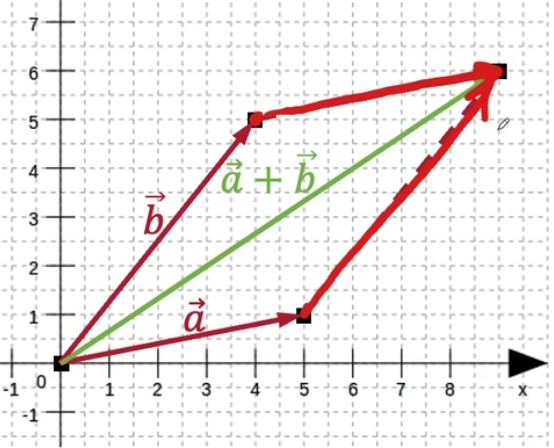
\includegraphics{Bilder/vector_add.png}
	\caption{Vektoraddition}
	\end{figure}
	\subsubsection{Multiplikation}
	\paragraphlb{Mite Skalar}
	Man kann einen Vektor auch multiplizieren, dabei diesen jedoch auch mit einem Skalar verbinden wobei jedes Element des Vektors mit diesem Skalar multipliziert wird: \textbf{a}*k=\vec{a}*k=\begin{pmatrix} $a_1*k$ \\ $a_2*k$ \\ $a_3*k$ \\ ... \\ $a_n*k$\end{pmatrix} \\
	\paragraphlb{Skalarprodukt}
	Wenn man zwei Vektoren miteinander multipliziert erhält man am Ende einen Skalar. Dabei wird jedes Element eines Vektors mit dessen Paar multipliziert, welche danach addiert werden. \textbf{a*b}=\vec{a}*\vec{b}=$a_1*b_1+a_2+b_2+...+a_n*b_n$. Das Skalarprodukt wird als $\vec{a}\cdot\vec{b}$ geschrieben
	\subsubsection{Gleichheit}
	Die Gleichheit von Vektoren ist gegeben wenn jedes Element eines Vektors gleich ist wie das passende Element des anderen Vektors: \textbf{a=b}$=a_1=a_2, a_2=a_3$
	\subsection{Beispiele}
	Gegeben: $\vec{a}=(x-1,2y,x+z), \vec{b}=(0,4,-1)$ \\
	Gesucht: Die reellen Zahlen x, y und z sodass $\vec{a}=\vec{b}$ \\
	$\vec{a}=\vec{b}=\begin{pmatrix} x-1 \\ 2y  \\ x+z \end{pmatrix}=\begin{pmatrix} 0 \\ 4 \\ -1  \end{pmatrix}$
	\subsubsection{Skalarprodukt}
	Gegeben: $\vec{a}=(1,3,5), \vec{b}=(2,0,4)$ \\
	Gesucht: $\vec{a}\cdot\vec{b}$ \\
	$\vec{a}\cdot\vec{b}=\begin{pmatrix} 1 \\ 3 \\ 5 \end{pmatrix}\cdot \begin{pmatrix} 2 \\ 0 \\ 4 \end{pmatrix}=1*2+3*0+5*4=2+0+20=22$
	\subsection{Vektorraum}
	Der Vektorraum ist wie bereits erwähnt die Gesamtheit aller Vektoren die die gleichen Eigenschaften besitzen (Die gleiche Menge an Elementen). In einem Raum gelten folgende Regeln:
	\subsubsection{Addition}
	\begin{itemize}
		\item{Kommutativität}
		\begin{itemize}
			\item{$\vec{a}+\vec{b}=\vec{b}+\vec{a}$}
		\end{itemize}
		\item{Assoziativität}
		\begin{itemize}
			\item{(\vec{a}+\vec{b})+\vec{c}?\vec{a}+(\vec{b}+\vec{c})}
		\end{itemize}
		\item{Neutrales Element}
		\item{Inverses Element}
	\end{itemize}
	\subsubsection{Multiplikation}
	\begin{itemize}
		\item{Assoziativität}
		\begin{itemize}
			\item{k(h \vec{a})=(kh)\vec{a}}
		\end{itemize}
		\item{Neutrales Element}
		\begin{itemize}
			\item{1 \vec{a}=\vec{a}}
		\end{itemize}
		\item{Distributivität}
		[TODO REGELN]
	\end{itemize}
	\subsection{Vektorlänge}
	Vektoren mit mehr als drei Komponenten lassen sich grafisch nur bedingt veranschaulichen, haben jedoch auch außerhalb von grafischer Darstellung einen Nutzen. Die Länge eines Vektors ist der Betrag dessen Komponenten. Also kann man mit dem Satz des Pythagoras die Länge eines Vektors bestimmen (Da die Länge eines Vektors die Hypothenuse eines gespannten Dreiecks ist.) $||\vec{a}||=\sqrt{a^2+b^2}$. \\
	Diese Regel ist auch für Vektoren mit mehr als 2 oder 3 Elementen anwendbar: $||\vec{a}||=\sqrt{\sum_{j=1}^{n}a_j^2=\sqrt{a_1^2+a_2^2+a_3^2+...+a_n^2}}$ \\
	Der Betrag ist immer eine nichtnegative reelle Zahl, selbst wenn der Vektor selbst negativ ist. Gleichzeitig ist der Betrag nur 0, wenn alle Elemente des Vektors 0 sind. \\
	Man kann dies auch verwenden um den Abstand zweier Punkte berechnen: $||\overrightarrow{AB}||=\sqrt{(B_1-A_1)^2+(B_2-A_2)^2+...+(B_N-A_N)^2}$ \\
	Im Falle des Abstands ist die Reihenfolge der Vektoren jedoch unwichtig. Ob man also A von B abzieht oder B von A führt zum gleichen Ergebnis.
	\subsection{Einheitsvektor}
	Ein Einheitsvektor ist ein Vektor mit der Länge 1. Ein Einheitsvektor eines beliebigen Vektors hat die selbe Richtung als dieser Vektor mit der Länge von 1. Diesen berechnet man indem man ihn durch die Inverse der Länge des Vektors dividiert: ${\frac{1}{||\vec{a}||}\vec{a}}$. Einheitsvektoren werden häufig bei Matrizenrechnungen verwendet
	\subsection{Vektornormen}
	Eine Vektornorm ist ein Raum in dem eine Norm definiert ist. Die Norm ist die Verallgemeinerung des geometrischen Begriffs der Länge: $||\cdot||:V\rightarrow [0, \infty)]$. Sie ordnet also jedem Element eines Vektorraums eine nichtnegative reelle Zahl zu. \\
	Normen müssen einige Bedingungen erfüllen:
	\begin{itemize}
		\item{Positivität - Jede Norm ist eine Positive Zahl (Ausnahme ist der Nullvektor)}
		\item{Definitheit - }
		\item{Absolute Homogenität - }
		\item{Subadditivität - Die Norm zweier addierter Vektoren ist definitiv kleiner (oder maximal gleich) als die Summe der Normen der separaten Vektoren}
	\end{itemize}
	\subsubsection{P-Norm}

	\paragraphlb{Betragssummennorm}
	Die Betragssummennorm, auch 1-Norm genannt ist eine p-Norm mit dem Wert 1: $||x||_1:=\sum_{i=1}^{n}|xi|$ \\
	Die Betragssummennorm eines Vektors ist die Summe des Betrags aller Komponenten eines Vektors. Das entspricht den Längen der Achsen des Vektors.
	\paragraphlb{Euklidische Norm}
	Die Euklidische Norm, auch 2-Norm genannt ist die gleiche Formel mit dem Wert 2: $||x||_2:=\sqrt{\sum_{i=1}^{n}}$. Das entspricht genau der Länge des Vektors selbst.
	\paragraphlb{Teschebyschow Norm}
	Hierbei wird das Maximum der Komponenten genommen. Dabei wird der Betrag jedes Elements eines Vektors herangezogen und das Maximum genommen. Wenn ein Vektor also die Werte 1, 2 und -3 enthält, wäre das Maximum 3, da der Betrag von -3 der höchste Wert ist. Das entspricht der einzelnen längsten Länge des Vektors.
	\subsection{Lineare Unabhängigkeit}
	Vektoren sind jeweils entweder linear abhängig oder unabhängig voneinander. Ein Vektor ist linear abhängig von einem anderen Vektor, wenn diese parallel zueinander stehen. Vektoren sind genau dann linear unabhängig wenn man in der Vektorgleichung $k_1 \overrightarrow{a_1}+k_2 \overrightarrow{a_2}+...+k_m \overrightarrow{a_m}=\vec{0}$ erhält, wobei jedes k gleich 0 ist und \textit{das die einzige Möglichkeit ist} um das Ergebnis zu erhalten. Falls das nicht möglich ist, sind zwei Vektoren linear abhängig. Auch wenn sich nur einer der Vektoren als Linearkombination schreiben lässt, sind diese linear abhängig. Per Definition ist auch ein Nullvektor linear abhängig.
	\subsubsection{Komplanar}
	Drei Vektoren sind abhängig, wenn sie in einer Ebene durch Verlängerung oder Verkürzung eine Ebene bilden. Im zweidimensionalen Raum sind ab einer gewissen Länge alle Vektoren komplanar. In einem dreidimensionalen Raum können Vektoren jedoch unabhängig sein, wenn sie in einer anderen Dimension stehen. \\
	Man kann Vektoren kombinieren, indem Vektoren mit beliebigen Skalaren verbunden werden. Dabei wird jeder Vektor mit einem Skalar multipliziert und danach aufaddiert. Das Resultat ist ein neuer Vektor. \\
	Um eine Linearkombination zu ermitteln, muss man für zwei Vektoren ein lineares Gleichungssystem bilden. [TODO Kombination] \\
	In diesem Fall existiert eine eindeutige Lösung. Das funktioniert, da diese beiden Vektoren linear unabhängig sind. Man kann für jeden beliebigen Vektor eine Lösung finden, falls die Vektoren linear unabhängig voneinander sind. \\
	Das funktioniert auch im dreidimensionalen Raum
	
































	\section{Matrizen}
	\section{Graphentheorie}

	























  
\end{document}